\documentclass[../main.tex]{subfiles}
\graphicspath{{\subfix{../images/}}, {\subfix{../}}}

\begin{document}

\chapter{Superconductivity}

\subsection{Extracting \(T_{\mathrm{C}}\)}

From Niklas \todo{Find a source for that! Phase transitions}

Übrigens: Typische Varianten, um `sauber(er)' Tc zu bestimmen, ist \(|OP|^2\) gegen \(T\) aufzutragen, da das (als Phasenübergang 2. Ordnung) proportional zu T-Tc ist.
Heißt, man kann Tc dann mittels linearem Fit finden - ist leider auch nicht immer der einfachste Weg, weil der Bereich, in dem diese lineare Näherung prinzipiell sehr klein um Tc herum sein kann.
Aber pi-mal-Daumen Abschätzungen gehen damit ganz gut.
Oder man macht es wie unten beschrieben mit einer daraus abgeleiteten Formel.

\begin{figure}
    \centering
    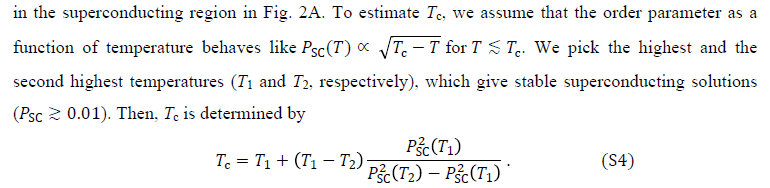
\includegraphics[width=\textwidth]{notes/images/getting T_C}
    \caption{Formula for extracting \(T_{\mathrm{C}}\)}
    \label{fig:Formula for extracting T_C}
\end{figure}

\end{document}
